\documentclass{beamer}\usepackage[]{graphicx}\usepackage[]{color}
%% maxwidth is the original width if it is less than linewidth
%% otherwise use linewidth (to make sure the graphics do not exceed the margin)
\makeatletter
\def\maxwidth{ %
  \ifdim\Gin@nat@width>\linewidth
    \linewidth
  \else
    \Gin@nat@width
  \fi
}
\makeatother

\definecolor{fgcolor}{rgb}{0.345, 0.345, 0.345}
\newcommand{\hlnum}[1]{\textcolor[rgb]{0.686,0.059,0.569}{#1}}%
\newcommand{\hlstr}[1]{\textcolor[rgb]{0.192,0.494,0.8}{#1}}%
\newcommand{\hlcom}[1]{\textcolor[rgb]{0.678,0.584,0.686}{\textit{#1}}}%
\newcommand{\hlopt}[1]{\textcolor[rgb]{0,0,0}{#1}}%
\newcommand{\hlstd}[1]{\textcolor[rgb]{0.345,0.345,0.345}{#1}}%
\newcommand{\hlkwa}[1]{\textcolor[rgb]{0.161,0.373,0.58}{\textbf{#1}}}%
\newcommand{\hlkwb}[1]{\textcolor[rgb]{0.69,0.353,0.396}{#1}}%
\newcommand{\hlkwc}[1]{\textcolor[rgb]{0.333,0.667,0.333}{#1}}%
\newcommand{\hlkwd}[1]{\textcolor[rgb]{0.737,0.353,0.396}{\textbf{#1}}}%
\let\hlipl\hlkwb

\usepackage{framed}
\makeatletter
\newenvironment{kframe}{%
 \def\at@end@of@kframe{}%
 \ifinner\ifhmode%
  \def\at@end@of@kframe{\end{minipage}}%
  \begin{minipage}{\columnwidth}%
 \fi\fi%
 \def\FrameCommand##1{\hskip\@totalleftmargin \hskip-\fboxsep
 \colorbox{shadecolor}{##1}\hskip-\fboxsep
     % There is no \\@totalrightmargin, so:
     \hskip-\linewidth \hskip-\@totalleftmargin \hskip\columnwidth}%
 \MakeFramed {\advance\hsize-\width
   \@totalleftmargin\z@ \linewidth\hsize
   \@setminipage}}%
 {\par\unskip\endMakeFramed%
 \at@end@of@kframe}
\makeatother

\definecolor{shadecolor}{rgb}{.97, .97, .97}
\definecolor{messagecolor}{rgb}{0, 0, 0}
\definecolor{warningcolor}{rgb}{1, 0, 1}
\definecolor{errorcolor}{rgb}{1, 0, 0}
\newenvironment{knitrout}{}{} % an empty environment to be redefined in TeX

\let\hlesc\hlstd \let\hlpps\hlstd \let\hllin\hlstd \let\hlslc\hlcom \let\hlppc\hlcom
\usepackage{alltt}

\title{Python Intro --- Part 2}
\subtitle{Spectrograms}
\author{Daniel Guest}
\IfFileExists{upquote.sty}{\usepackage{upquote}}{}
\begin{document}

\maketitle

\tableofcontents

\section{KnitR}

\begin{frame}[fragile]
\frametitle{First, a small aside...}
\begin{itemize}
	\item This entire presentation is a KnitR demonstration, as well as a presentation on Python

	\item Check out the .Rnw file to see the mixture of \LaTeX{} code and R code that is Sweaved together by KnitR to generate the output
	
	\item I'm using the \LaTeX{} beamer package to create this slideshow

	\item KnitR makes for very elegant presentations of R code and easy inclusion of graphics
\end{itemize}
\end{frame}

\begin{frame}[fragile]
\frametitle{First, a small aside...}


\begin{knitrout}
\definecolor{shadecolor}{rgb}{0.969, 0.969, 0.969}\color{fgcolor}\begin{kframe}
\begin{alltt}
\hlstd{d} \hlkwb{<-} \hlkwd{select}\hlstd{(iris, Sepal.Width, Petal.Length, Petal.Width)}
\hlkwd{head}\hlstd{(d)}
\end{alltt}
\begin{verbatim}
##   Sepal.Width Petal.Length Petal.Width
## 1         3.5          1.4         0.2
## 2         3.0          1.4         0.2
## 3         3.2          1.3         0.2
## 4         3.1          1.5         0.2
## 5         3.6          1.4         0.2
## 6         3.9          1.7         0.4
\end{verbatim}
\end{kframe}
\end{knitrout}
\end{frame}

\begin{frame}[fragile]
\frametitle{First, a small aside...}

\begin{knitrout}
\definecolor{shadecolor}{rgb}{0.969, 0.969, 0.969}\color{fgcolor}\begin{kframe}
\begin{alltt}
\hlkwd{ggplot}\hlstd{(d,}\hlkwd{aes}\hlstd{(}\hlkwc{x}\hlstd{=Sepal.Width,} \hlkwc{y}\hlstd{=Petal.Length,} \hlkwc{color}\hlstd{=Petal.Width))} \hlopt{+} \hlkwd{geom_point}\hlstd{()}
\end{alltt}
\end{kframe}
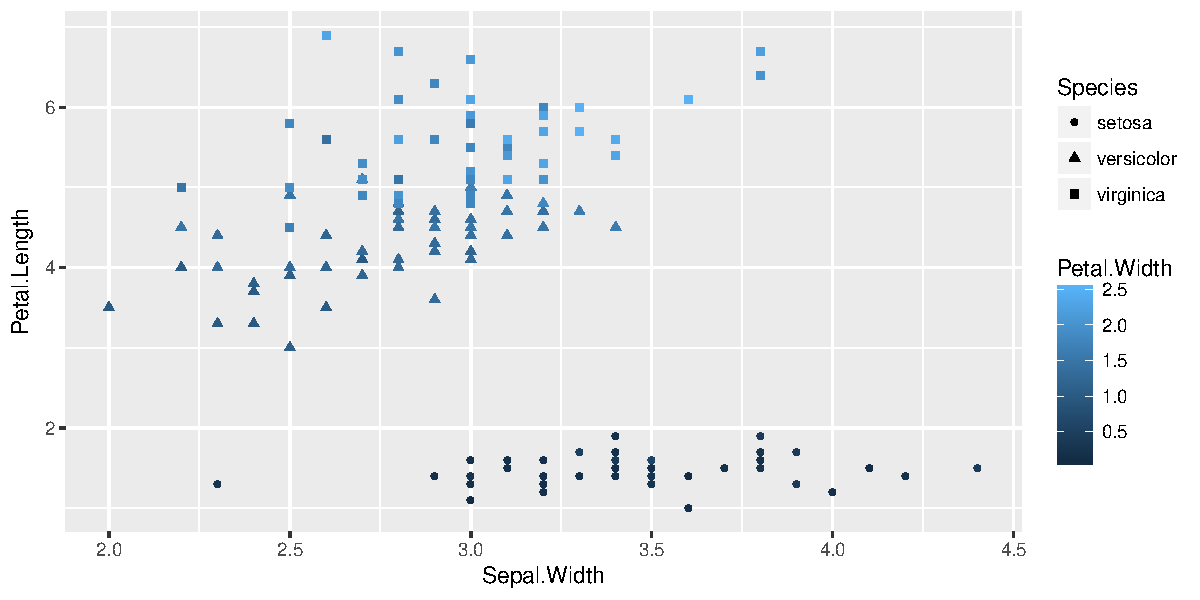
\includegraphics[width=\maxwidth]{figure/unnamed-chunk-3-1} 

\end{knitrout}
\end{frame}

\begin{frame}[fragile]
\frametitle{First, a small aside...}

\begin{itemize}
	\item Of course, the question arises --- Why is KnitR and \LaTeX{} in this presentation?

	\item KnitR is also ready to handle other languages

	\item If you ever need to present code in Python, C, R, Scala, Perl, Fortran, etc...

	\item For example...

\begin{knitrout}
\definecolor{shadecolor}{rgb}{0.969, 0.969, 0.969}\color{fgcolor}\begin{kframe}
\noindent
\ttfamily
\hlstd{x\ }\hlopt{=\ {[}}\hlstd{}\hlnum{1}\hlstd{}\hlopt{,}\hlstd{}\hlnum{2}\hlstd{}\hlopt{,}\hlstd{}\hlnum{3}\hlstd{}\hlopt{,}\hlstd{}\hlnum{4}\hlstd{}\hlopt{,}\hlstd{}\hlnum{5}\hlstd{}\hlopt{{]}}\hspace*{\fill}\\
\hlstd{x}\hlopt{.}\hlstd{}\hlkwd{append}\hlstd{}\hlopt{(}\hlstd{}\hlnum{4}\hlstd{}\hlopt{)}\hspace*{\fill}\\
\hlstd{}\hlkwa{print}\hlstd{}\hlopt{(}\hlstd{}\hlnum{2}\hlstd{}\hlopt{+}\hlstd{}\hlnum{2}\hlstd{}\hlopt{)}\hspace*{\fill}\\
\hlstd{}\hlkwa{print}\hlstd{}\hlopt{(}\hlstd{x}\hlopt{)}\hlstd{}\hspace*{\fill}
\mbox{}
\normalfont

\begin{verbatim}
## 4
## [1, 2, 3, 4, 5, 4]
\end{verbatim}
\end{kframe}
\end{knitrout}
\end{itemize}
\end{frame}

\section{Intro}

\begin{frame}
\frametitle{Plan}
\begin{itemize}
	\item We're going to focus on two things today

	\begin{enumerate}
		\item Theoretical --- control statements and loops

		\item Practical --- applying numpy and scipy to analyze sound 
	\end{enumerate}

	\item What we'll need
	\begin{enumerate}
		\item Python 3 (through IPython)

		\item numpy, scipy, matplotlib, sounddevice

		\item Sound files (in folder "samples") 
	\end{enumerate}

	\item Overview
	\begin{enumerate}
		\item Set up scripting tools

		\item A brief intro to loops

		\item Make one spectrogram

		\item Make a bunch of spectrograms
	\end{enumerate}
\end{itemize}
\end{frame}

\section{Scripts}

\begin{frame}
\frametitle{Bare bones scripting}
\begin{itemize}
	\item Today, we'll set up a bare bones environment for scripts

	\item You'll soon probably want something more fully fledged...
	\begin{enumerate}
		\item Spyder

		\item Eclipse
	\end{enumerate}

	\item Now, let's open up Notepad++
\end{itemize}
\end{frame}

\section{Loops}

\begin{frame}[fragile]
\frametitle{Our first loop}
\begin{itemize}
	\item Loops in Python have a very easy and powerful syntax

\end{itemize}
\begin{knitrout}
\definecolor{shadecolor}{rgb}{0.969, 0.969, 0.969}\color{fgcolor}\begin{kframe}
\noindent
\ttfamily
\hlstd{}\hlkwa{for\ }\hlstd{i\ }\hlkwa{in\ }\hlstd{}\hlkwb{range}\hlstd{}\hlopt{(}\hlstd{}\hlnum{5}\hlstd{}\hlopt{):}\hspace*{\fill}\\
\hlstd{\ }\hlkwa{print}\hlstd{}\hlopt{(}\hlstd{i}\hlopt{)}\hlstd{}\hspace*{\fill}
\mbox{}
\normalfont

\begin{verbatim}
## 0
## 1
## 2
## 3
## 4
\end{verbatim}
\end{kframe}
\end{knitrout}

\end{frame}

\begin{frame}[fragile]
\frametitle{Loop syntax}
\begin{itemize}
	\item Unlike MATLAB and R which employ brackets, Python uses tabs to indicate nesting

	\item If we don't nest at least one line for a loop we'll have problems

	\item I personally like this, I think it promotes more readable code!

\end{itemize}
\begin{knitrout}
\definecolor{shadecolor}{rgb}{0.969, 0.969, 0.969}\color{fgcolor}\begin{kframe}
\noindent
\ttfamily
\hlstd{}\hlkwa{for\ }\hlstd{i\ }\hlkwa{in\ }\hlstd{}\hlkwb{range}\hlstd{}\hlopt{(}\hlstd{}\hlnum{5}\hlstd{}\hlopt{):}\hspace*{\fill}\\
\hlstd{}\hlkwa{print}\hlstd{}\hlopt{(}\hlstd{i}\hlopt{)}\hlstd{}\hspace*{\fill}
\mbox{}
\normalfont

\begin{verbatim}
##   File "<string>", line 2
##     print(i)
##         ^
## IndentationError: expected an indented block
\end{verbatim}
\end{kframe}
\end{knitrout}

\end{frame}


\begin{frame}[fragile]
\frametitle{Looping over other things}
\begin{itemize}
	\item We can loop over a variety of objects

	\item The range() function is for when we want integer sequences, but many things in Python can be used to create a loop (technically, these things are called iterables in Python-lingo)

	\item Lists are iterables...

\end{itemize}
\begin{knitrout}
\definecolor{shadecolor}{rgb}{0.969, 0.969, 0.969}\color{fgcolor}\begin{kframe}
\noindent
\ttfamily
\hlstd{x\ }\hlopt{=\ {[}}\hlstd{}\hlnum{1}\hlstd{}\hlopt{,}\hlstd{}\hlnum{4}\hlstd{}\hlopt{,}\hlstd{}\hlnum{9}\hlstd{}\hlopt{,}\hlstd{}\hlnum{16}\hlstd{}\hlopt{,}\hlstd{}\hlnum{25}\hlstd{}\hlopt{{]}}\hspace*{\fill}\\
\hlstd{}\hlkwa{for\ }\hlstd{i\ }\hlkwa{in\ }\hlstd{x}\hlopt{:}\hspace*{\fill}\\
\hlstd{\ }\hlkwa{print}\hlstd{}\hlopt{(}\hlstd{}\hlkwb{str}\hlstd{}\hlopt{(}\hlstd{i}\hlopt{)\ +\ }\hlstd{}\hlkwb{str}\hlstd{}\hlopt{(}\hlstd{x}\hlopt{))}\hlstd{}\hspace*{\fill}
\mbox{}
\normalfont

\begin{verbatim}
## 1[1, 4, 9, 16, 25]
## 4[1, 4, 9, 16, 25]
## 9[1, 4, 9, 16, 25]
## 16[1, 4, 9, 16, 25]
## 25[1, 4, 9, 16, 25]
\end{verbatim}
\end{kframe}
\end{knitrout}

\end{frame}

\begin{frame}[fragile]
\frametitle{Looping over other things}
\begin{itemize}
	\item Strings are also iterables... 

\end{itemize}
\begin{knitrout}
\definecolor{shadecolor}{rgb}{0.969, 0.969, 0.969}\color{fgcolor}\begin{kframe}
\noindent
\ttfamily
\hlstd{}\hlkwa{for\ }\hlstd{i\ }\hlkwa{in\ }\hlstd{}\hlstr{"Hello"}\hlstd{}\hlopt{:}\hspace*{\fill}\\
\hlstd{\ }\hlkwa{print}\hlstd{}\hlopt{(}\hlstd{i}\hlopt{)}\hlstd{}\hspace*{\fill}
\mbox{}
\normalfont

\begin{verbatim}
## H
## e
## l
## l
## o
\end{verbatim}
\end{kframe}
\end{knitrout}
\end{frame}

\section{Making a spectrogram}
\begin{frame}[fragile]
\frametitle{Setting up the environment}
\begin{itemize}
	\item First, we need to import the necessary modules
\begin{knitrout}
\definecolor{shadecolor}{rgb}{0.969, 0.969, 0.969}\color{fgcolor}\begin{kframe}
\noindent
\ttfamily
\hlstd{}\hlkwa{import\ }\hlstd{numpy}\hspace*{\fill}\\
\hlkwa{from\ }\hlstd{scipy}\hlopt{.}\hlstd{io\ }\hlkwa{import\ }\hlstd{wavfile}\hspace*{\fill}\\
\hlkwa{import\ }\hlstd{matplotlib}\hlopt{.}\hlstd{pyplot\ }\hlkwa{as\ }\hlstd{plt}\hspace*{\fill}
\mbox{}
\normalfont
\end{kframe}
\end{knitrout}
\end{itemize}

\begin{itemize}
	\item Numpy --- provides key matrix and DSP operations

	\item wavfile --- provides read/write to wavfile
	
	\item pyplot --- user-friendly functions and objects for plotting
\end{itemize}
\end{frame}

\end{document}
